\mydet{\vec{V}&\vec{u}\\\vec{u}^T&f} of \eqref{eq:solutions/13/3/1} becomes
\begin{align}
    \mydet{-3&-4&-\frac{29}{2}\\-4&3&\frac{3}{2}\\-\frac{29}{2}&\frac{3}{2}&-18}\label{eq:solutions/13/3/2}
\end{align}
Expanding equation \eqref{eq:solutions/13/3/2}, we get zero.\\
Hence given equation represents a pair of straight lines.
Slopes of the individual lines are roots of equation 
\begin{align}
    cm^2+2bm+a=0\\
    \implies 3m^2-8m-3=0\\
    \text{Solving, }m=3,-\frac{1}{3}
\end{align}
The normal vectors of the lines then become
\begin{align}
    \vec{n_1}=\myvec{\frac{1}{3}\\1}\\
    \vec{n_2}=\myvec{-3\\1}
\end{align}
Equations of the lines can therefore be written as
\begin{align}
  \myvec{\frac{1}{3}&1}\vec{x}=c\\
 \implies \myvec{1&3}\vec{x}=c_1 ,\\
   \myvec{-3&1}\vec{x}=c_2\\
  \implies \left[\myvec{1&3}\vec{x}-c_1\right]\left[\myvec{-3&1}\vec{x}-c_2\right]
\end{align}
represents the equation specified in \eqref{eq:solutions/13/3/1}\\
Comparing the equations, we have
\begin{align}
    \myvec{1&-3\\3&1}\myvec{c_2\\c_1}=\myvec{29\\-3}\\
 \end{align}
 Row reducing the augmented matrix
 \begin{align}
    \myvec{1&-3&29\\3&1&-3}\xleftrightarrow[]{R_2\leftarrow R_2-3\times R_1}
    \myvec{1&-3&29\\0&10&-90}\\
    \xleftrightarrow[]{R_2\leftarrow R_2\times \frac{1}{10}}
    \myvec{1&-3&29\\0&1&-9}\\
    \xleftrightarrow[]{R_1\leftarrow R_1+3\times R_2}
    \myvec{1&0&2\\0&1&-9}\\
    \implies c_2=2 \text{ and }c_1=-9
\end{align}
The individual line equations therefore become
\begin{align}
    \myvec{1&3}\vec{x}=-9\label{eq:solutions/13/3/3} ,\\\myvec{-3&1}\vec{x}=2\label{eq:solutions/13/3/4}
\end{align}
Note that the convolution of the normal vectors, should satisfy the below condition
\begin{align}
    \myvec{1\\3}*\myvec{-3\\1}=\myvec{a\\2b\\c}\label{eq:solutions/13/3/5}
\end{align}
The LHS part of \eqref{eq:solutions/13/3/5} can be rewritten using toeplitz matrix as
\begin{align}
    \myvec{1&0\\3&1\\0&3}\myvec{-3\\1}=\myvec{-3\\-8\\3}=\myvec{a\\2b\\c}
\end{align}

The augmented matrix for the set of equations represented in \eqref{eq:solutions/13/3/3}, \eqref{eq:solutions/13/3/4} is
\begin{align}
\myvec{1&3&-9\\-3&1&2}
\end{align}
Row reducing the matrix
\begin{align}
 \myvec{1&3&-9\\-3&1&2}\xleftrightarrow[]{R_2\leftarrow R_2+3\times R_1}\myvec{1&3&-9\\0&10&-25}\\
 \xleftrightarrow[]{R_1\leftarrow R_1-\frac{3}{10}\times R_2}\myvec{1&0&-\frac{3}{2}\\0&10&-25}\\
 \xleftrightarrow[]{R_2\leftarrow \frac{R_2}{10}}\myvec{1&0&-\frac{3}{2}\\0&1&-\frac{5}{2}}\\
\text{Hence, the intersection point is}
\myvec{-\frac{3}{2}\\-\frac{5}{2}}
\end{align}
\begin{figure}[!ht]
\centering
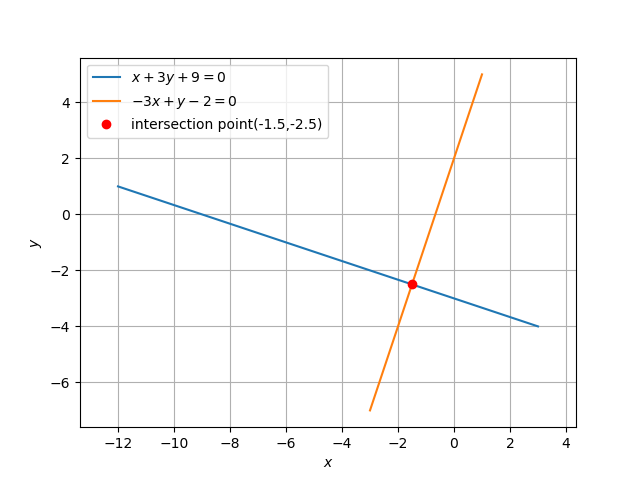
\includegraphics[width=\columnwidth]{./solutions/13/3/hw4plot.png}
\caption{plot showing intersection of lines}
\label{eq:solutions/13/3/Fig:solutions/13/3/}
\end{figure}
Angle between two lines $\theta$ can be given by
\begin{align}
\cos \theta = \frac{\vec{n_1}^T\vec{n_2}}{\norm{\vec{n_1}}\norm{\vec{n_2}}}
\end{align}
%From \eqref{eq:solutions/13/3/3}, \eqref{eq:solutions/13/3/4},
\begin{align}
\cos \theta=\frac{\myvec{1&3}\myvec{-3\\1}}{\sqrt{(3)^2 +1} \times \sqrt{(-3)^2 +1}}=0\\
\implies \theta = 90\degree
\end{align}

